\cleardoublepage
\chapternonum{修改说明}
\noindent
尊敬的评审专家:

您好!

感谢您在百忙之中抽出时间仔细审阅我的论文,指出论文中写作内容与逻辑上的不足,并且给出很多宝贵的修改意见。在收到您严谨而又细致的评审意见之后,我第一时间和我导师
进行了探讨,并结合您的意见对论文进行了相应的修改,所有修改之处均使用红色字体进行了突出显示。在您再次开始评阅论文前,请允许我针对您的评审意见,对此次修改的具体内容进行介绍:

\textbf{一、\autoref{equ:maxap}缺“比较符号”,对\autoref{equ:maxap}的说明可以表达得更准确一些。}

感谢您的细致评审!\autoref{equ:maxap}中确实缺少比较符号,新修论文已经对其进行了更正。另外,本次修改也对全文各章的公式进行了再次检查,
防止类似错误再次发生。与此同时,本次修改后正文对\autoref{equ:maxap}的说明也进行了一定的拓展解释,详细内容烦请参阅论文$P5$。

\textbf{二、$P11$给出了比较NN和DL方法在PE预测方面应用的文献,该段描述的最后一句话“而使用NN算法时,模型识别的准确性亦可高达96.7\%。”中的“而..., ...亦...”表达不够准确,
也没有进一步讨论为什么NN比DL方法取得了更高的准确率,以为后续方法的选择奠定基础。}

正文此处引用了同一作者团队在2018年发表的两篇论文(1篇会议论文,1篇期刊论文)中的相关结论,在再次阅读文献后发现,两篇文献中的准确性数值略有出入。
本次修订以其中的期刊文章为标准对此处的相关结论进行了更正。更正后的版本没有使用“而..., ...亦...”的表达方式,同时也简单讨论了可能引起DL较NN算法训练所得的模型具有
更高准确性的原因。详细内容烦请参阅论文$P11$。

\textbf{三、$P17$中“UTRI”在首次出现时,应给出全称,以与文中其他符号的表述相一致。}

在本论文中,UTRI是uterine artery resistance index的缩写,其中文含义为子宫动脉阻力指数。由于UTRI在论文中首次出现的位置是在正文$P6$,论文
已在此处进行了标注,故$P17$再次出现未对其进行标注。另外,为方便评审,论文在写作伊始就将其中出现过的较为重要的英文缩写词进行汇总整理,即缩写词表(字母序)与
缩写词表(页码序)。

\textbf{四、文中PPG波形特征“重博波”应修改为“重搏波”,文中多处“搏”写成了“博”。}

感谢您的细致评审!此处的文字错误已经进行了全文修改。

\textbf{五、文中多处出现错字、漏字、少字、多字现象以及符号错误,请查找修改。}

感谢您的细致评审!论文在再次送审前已被打印并认真校对过,这些表达问题已经经过全文修改。请您再次审阅!

\textbf{六、\autoref{equ:AF6}中反映出了指端血液容积变化率不仅与光强变化率有关,也反映出其变化程度与输入光强有关,如何去除入射光强对最终结果的影响?}

\autoref{equ:AF6}反映出了指端血液容积变化率与光强变化率有关,即
\begin{equation}
    \frac{\Delta V_{a}}{V_{a}}=\frac{1}{\ln(I/I_{0})}\frac{\Delta I}{I}
\end{equation}
其中,$I_{0}$为入射光强度。在工程应用进行PPG的测量时,在一个完整的测量周期内,只需将入射光强度保持不变,即可消除上式中$I_{0}$对结果的影响。
考虑此处表述在原稿中存在一定的不精确,此次修改也进行了更正,详情参阅正文$P27$。

% 另外,在校对PPG信号的测量原理小节的公式时,发现\autoref{equ:AF2}、\autoref{equ:AF3}、\autoref{equ:AF4}与\autoref{equ:AF6}等遗漏了常数项,这些遗漏也在此次修稿中得到更正
% (这些常数项的遗漏不影响本章节涉及的公式推导及最终结论)。

\textbf{七、\autoref{equ:QS2}表示的应该是“第二个弹性腔室”的血液输入输出关系。}

感谢您的细致评审!此处的文字错误已经进行了修改。

\textbf{八、\autoref{equ:malpf}截止频率的下标与公式上面的文字描述保持一致。3.2.3所述PPG信号
采样率为100Hz,$P45$按照\autoref{equ:malpf}所计算的滤波器截止频率达到了89Hz,检查是否正确?另外,该部分出现多字问题。}

感谢您的细致评审!\autoref{equ:malpf}的标记已经从$f_{co}$修改为$f_{c}$。使用$N$=5的平滑滤波器对原始PPG信号进行处理,
按照\autoref{equ:malpf}所计算的滤波器截止频率应为8.9Hz,这一错误也已更正。为方便理解,此处相关描述文字进行了微调,详细内容烦请参阅论文$P45$。

\textbf{九、\autoref{equ:rpeak}所示波峰相对位置公式是否正确?分子分母是否反了?而\autoref{tab:checkingp}给出了判为有效波形均值相对区间的R值范围为[0.8,1.2]是否合适?}

感谢您的细致评审!\autoref{equ:rpeak}即
\begin{equation}
    \label{equ:rpeak0}
    R = \frac{n}{n_p}
\end{equation}
其中,$R$为当前PPG波形的波峰相对位置,$n$为该波形的采样点数,$n_p$为该波形波峰所对应的采样点下标值。
若交换上式中分子分母位置,得到
\begin{equation}
    \label{equ:rpeak1}
    R^{'} = \frac{n_p}{n}
\end{equation}
仔细观察\autoref{equ:rpeak0}与\autoref{equ:rpeak1}后,可以发现两式均可以表征PPG波形的波峰相对位置,其区别主要体现在两者的值域不同。由于
$0<n_p<n$,因此理论上$R$的值域为$(1, \infty)$,而$R^{'}$的值域为$(0,1)$。考虑到\autoref{equ:rpeak0}与\autoref{equ:rpeak1}并无实质性的区别,因而在论文写作时仅从中选取了\autoref{equ:rpeak0},
即正文中的\autoref{equ:rpeak}。

在正文$P49$已经阐述过这些复核标准的设计初衷,就是区分正常PPG波形与畸变波形,即使二者在这些复核表征上存在数值的差异。
与此同时,即便是来自同一个体不同的正常PPG波形按复核标准进行计算时也可能出现一定的数值差异。为进行有效波形的判断,论文在$P51$给出了下列处理策略:

1)计算当前个体的所有PPG波形对应的特征值。

2)将步骤1中所有数值排序后,选取部分数值计算均值。

3)依次将所有特征值与该均值进行比较,若特征值在均值的一定区间内,对应的波形才会被判断为有效波形(输出0);否则会被判为异常干扰(输出1)。

在上述过程中,SCD算法使用的复核标准的各超参数如\autoref{tab:checkingp}所示,其中与R对应的均值有效区间为[0.8,1.2]。
由于该区间并不是R值的直接反映,与其值域$(1, \infty)$并不冲突。此外,该均值有效区间也在SCD算法的实际检测中得到应用,检测结果也表明取值较为合理。

\textbf{十、在算法的决策阶段,不同复核标准的权重是如何确定的?}

SCD算法的设计初衷即为利用正常PPG波形与畸变波形在特定复核表征上的数值差异将二者进行区分。因此,如正文$P46$阐述的,
SCD算法可以视为一个广义上的监督学习模型的训练与应用过程$^{[133]}$。其中,多种形态学特征的复核结果对应着模型的输入数据,决策阶段使用的策略对应着模型的训练算法,
确定有效波形的决策过程则对应着模型在新数据集上的应用过程。而复核与决策阶段涉及的多项具体数值可以视为该模型的超参数。

而对一个监督学习来说,其模型超参数的训练依赖于训练集数据。而在SCD算法的超参数调参过程中,也是利用了部分原始数据构成训练集再进行超参数的调整与训练。
而在过程中,复核阶段与决策阶段的各项超参数(包括复核阶段的权重)均是在训练集的基础上得到的。与普通的仅需观察预测标签与实际标签是否一致的监督学习不同,对SCD算法的
校验还需结合波形的具体形态,特别是畸变波形的形态。这是由于畸变波形的识别直接影响了SCD算法的整体识别准确率。而论文中SCD算法的超参数就是基于训练集数据,在这个繁琐的过程中不断调整得到的。

综上,论文在正文$P46$、$P47$等处对上述超参数的确定过程进行了修改与补充。

\textbf{十一、PPG数据采样率提升到2000Hz的必要性?----PPG时域特征}

通常而言,在绘制PPG等电生理信号习惯性采用折线图,如图\autoref{fig:ep11}所示。而当我们采用散点图绘制对该波形
重新绘制后,可以观察到PPG信号被折线图所掩盖的更多细节信息,如图\autoref{fig:ep12}所示。可以看到PPG波形上升支较下降支具有更少、更稀疏的采样点。
当对PPG波形按\autoref{fig:all_views}展示的策略进行切割计算时,在原始信号只有100Hz的采样率下,可以发现切割线与波形交点的无法确定其具体幅值,如图\autoref{fig:ep13}所示。
这也导致了本论文提出的多种基于面积、幅值等角度的新型PPG形态学参数无法精确计算。而在通过插值方法提高采样率至2000Hz后,切割线与波形交点是可以确定其具体幅值的,如图\autoref{fig:ep14}所示。
因此,本论文在开始计算PPG波形的各项特征前,将数据采样率提高至2000Hz。

\begin{figure}[htbp]
    \centering
    \subfigure[\label{fig:ep11}PPG波形(100Hz)的折线图]{
    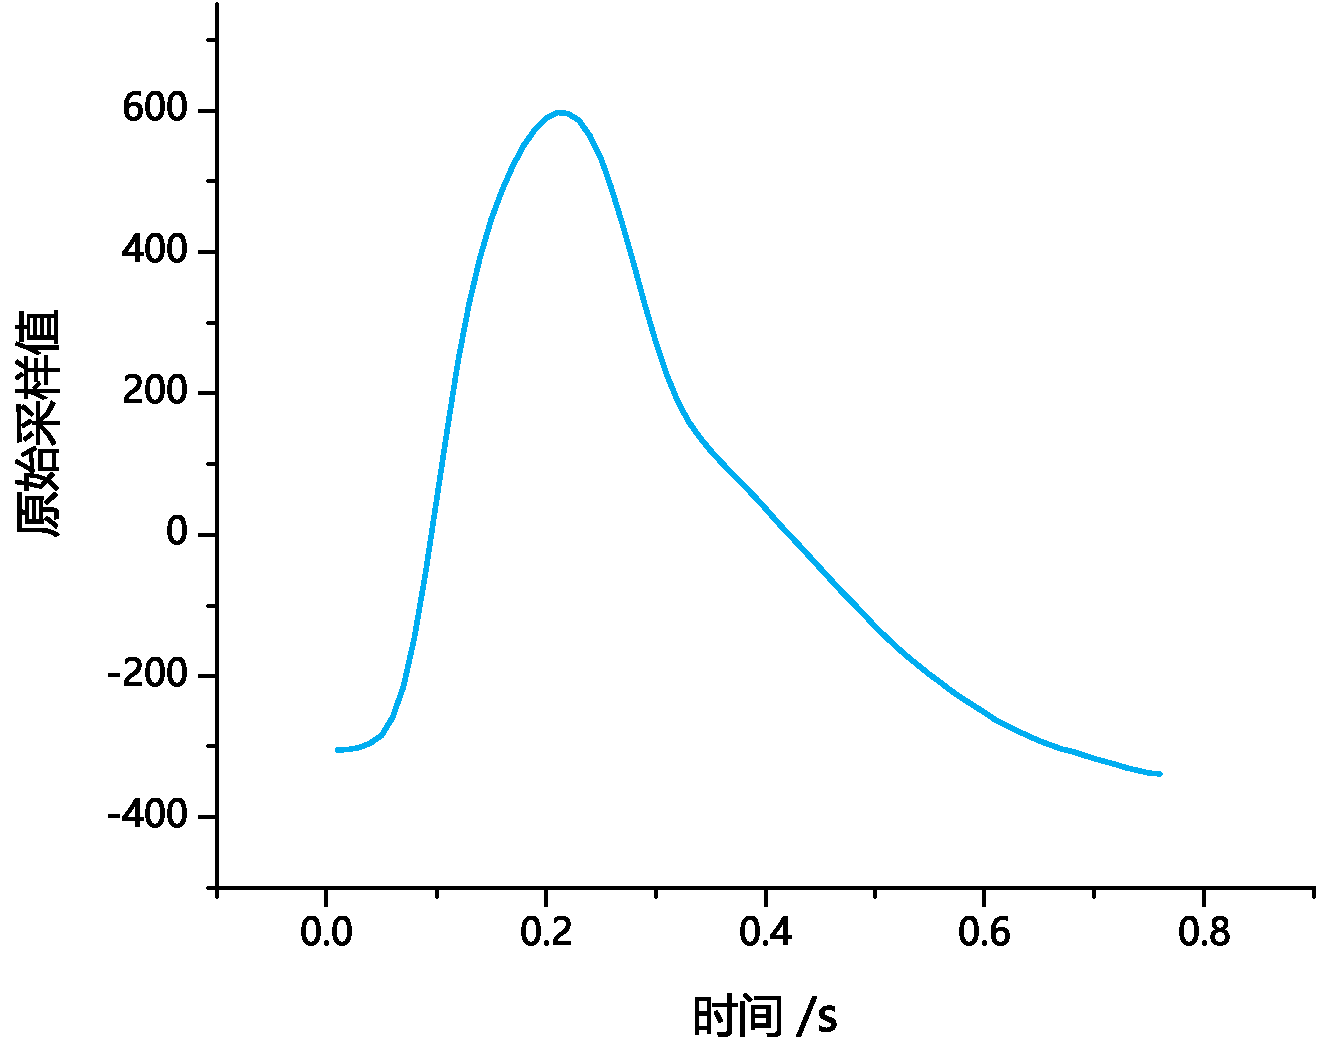
\includegraphics[width=6cm]{explain/01}
    }
    \quad
    \subfigure[\label{fig:ep12}PPG波形(100Hz)的散点图]{
    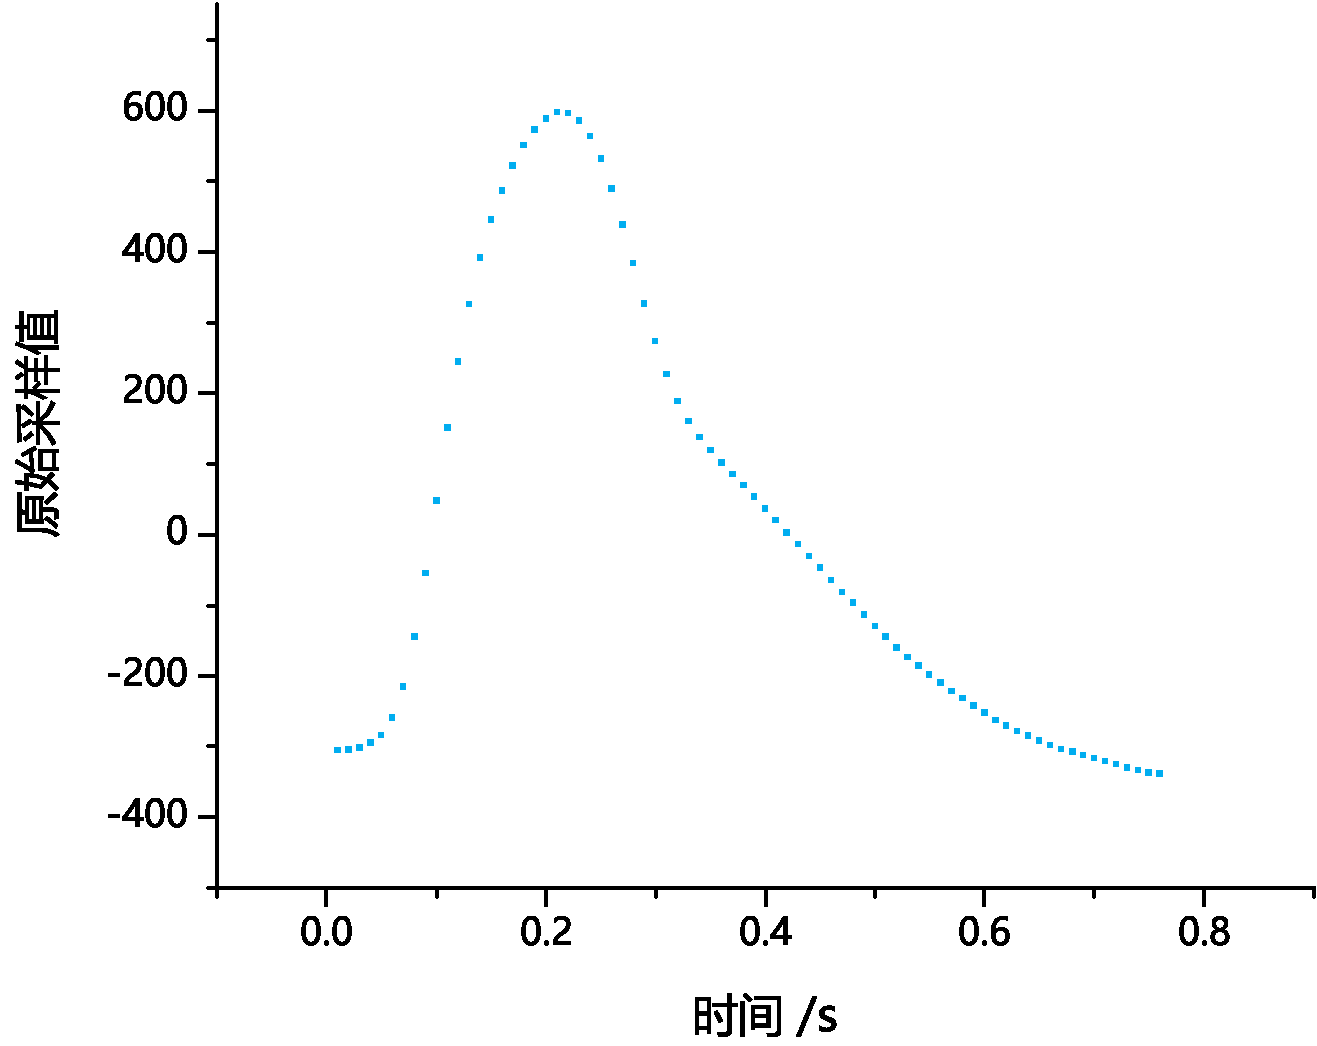
\includegraphics[width=6cm]{explain/02}
    }
    \quad
    \subfigure[\label{fig:ep13}对PPG波形(100Hz)进行切割处理]{
    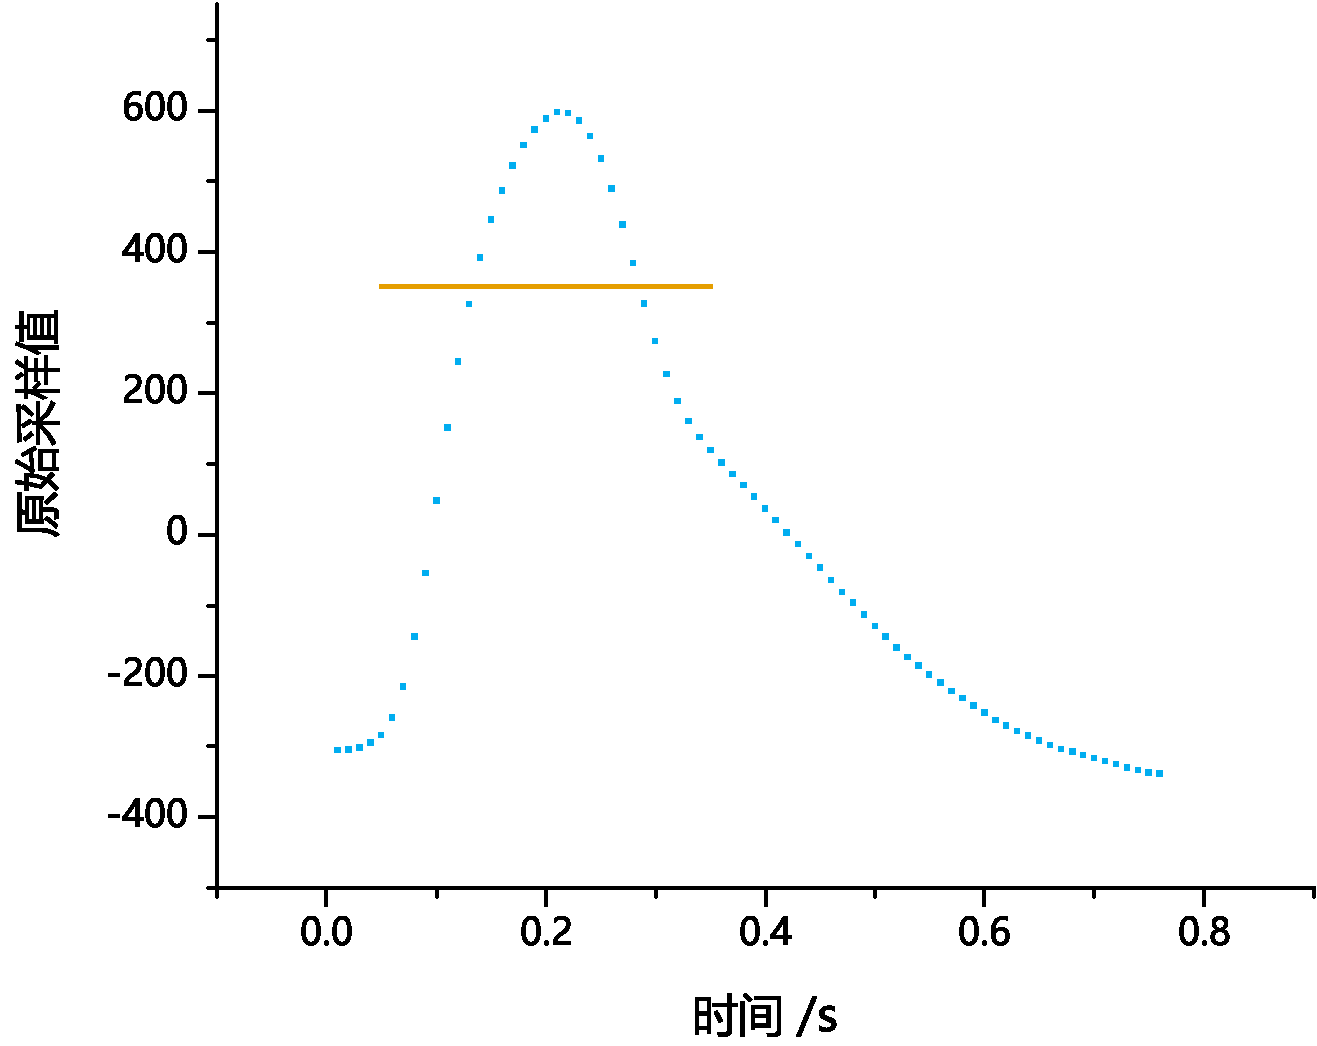
\includegraphics[width=6cm]{explain/03}
    }
    \quad
    \subfigure[\label{fig:ep14}对PPG波形(2000Hz)进行切割处理]{
    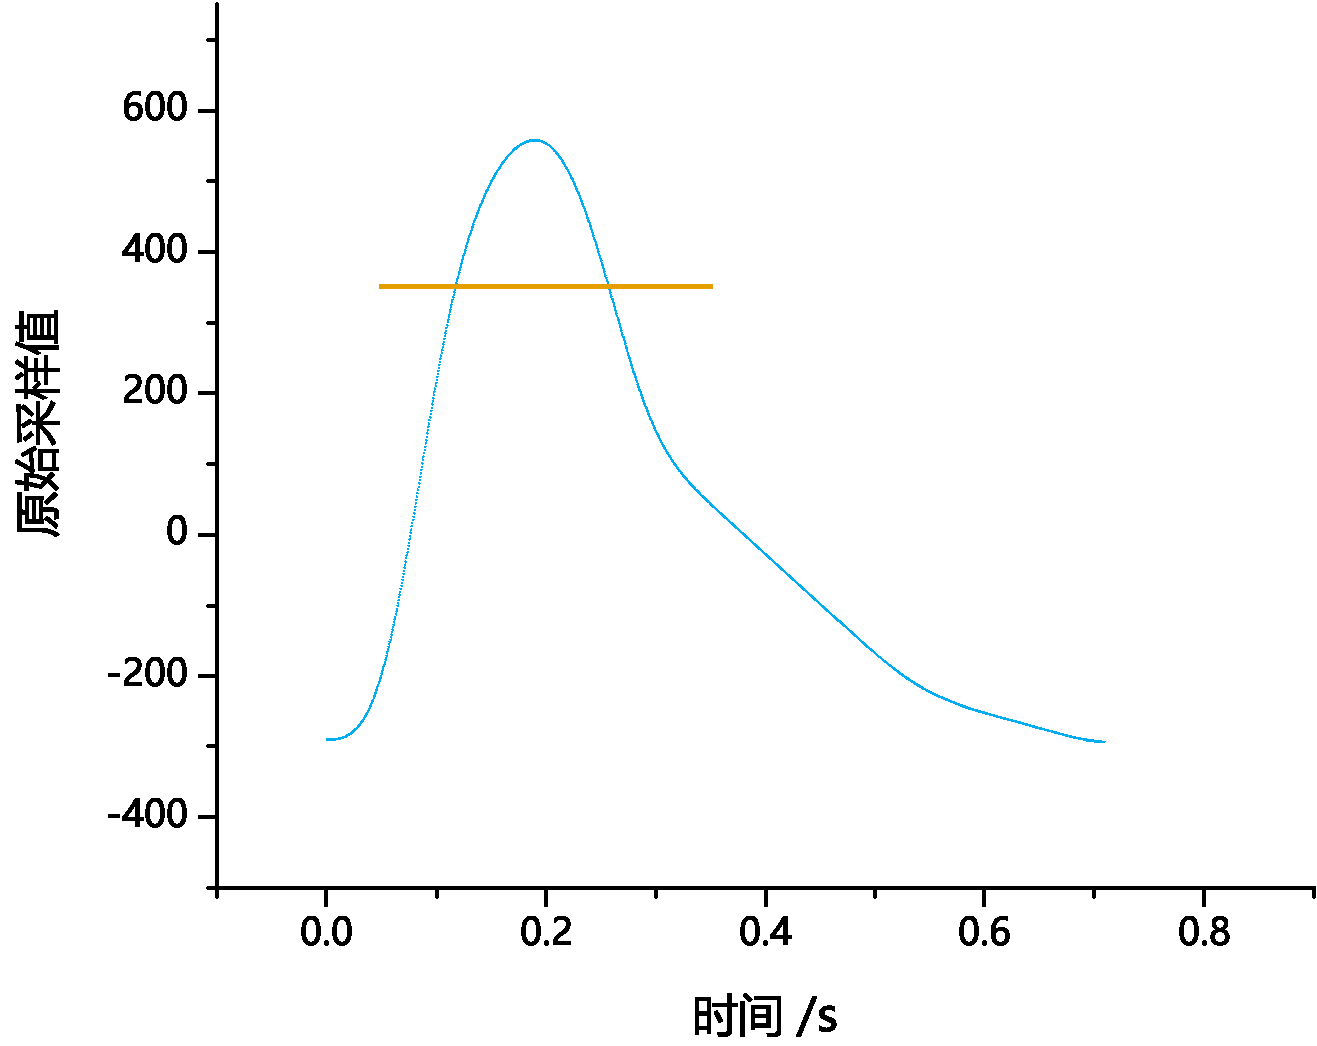
\includegraphics[width=6cm]{explain/04}
    }
    \caption[]{\label{fig:ep1}提高PPG采样率原理示意图}
\end{figure}

\textbf{十二、3.4.6提到“PPG信号波形幅值对不同个体而言并无实际的生理意义”,而\autoref{fig:frameworks3}给出的PPG的时域特征包含了“幅值类”特征,特别是后面提到的主波峰幅值、降
中峡幅值等,其作用是什么?}

感谢您的细致评审!关于这一问题的回复,我想从以下三个方面来回答:

1、关于PPG信号波形幅值对不同个体而言并无实际的生理意义

在第二章中已经阐述过,PPG本身是人体指端血液容积变化率的体现。且由于人体指端血液容积因人而异,不同个人的PPG的幅值大小没有绝对意义,因此也没有可比性。
本论文采集的不同个体的PPG数据的波形图也直接说明了这一点,如\autoref{fig:ep2}所示。
\begin{figure}[htbp]
    \centering
    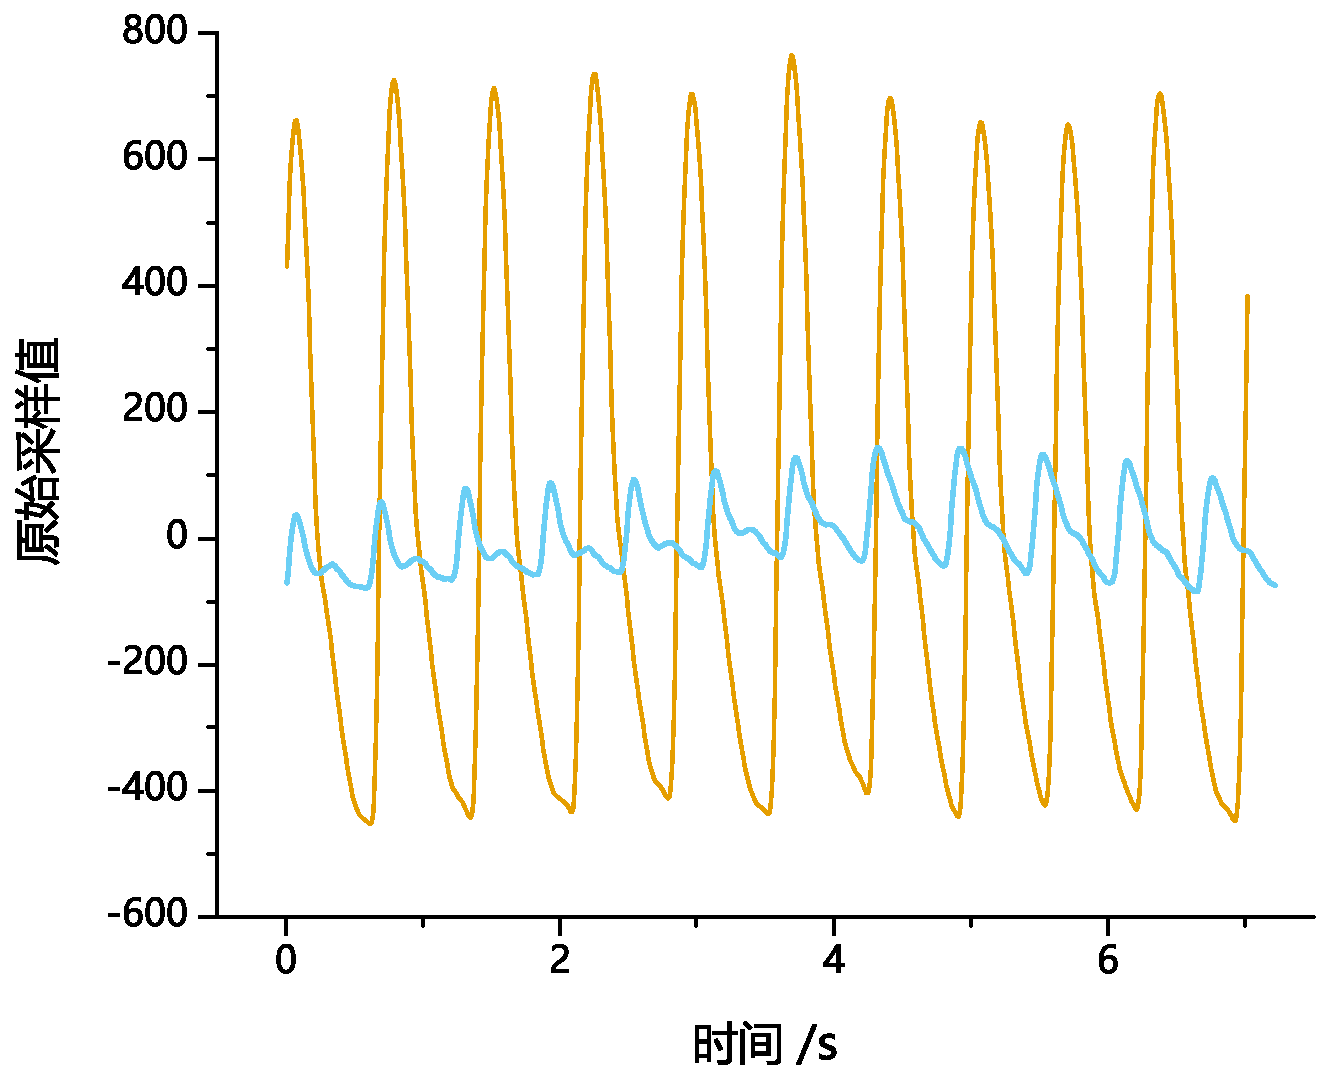
\includegraphics[width=.6\linewidth]{explain/05}
    \caption[]{\label{fig:ep2}不同个体的PPG波形对比图}
\end{figure}

2、3.5小节脉搏波的时域特征在论文中的作用

论文在绪论的1.3.5小节中介绍了多种PPG的时域参数,也介绍了这些参数在相关研究中的具体应用情况。考虑到文章篇幅与论文整体结构,这些时域参数的具体定义及其计算方式
并没有在1.3.5小节中进行介绍,而是在3.5小节中完成。
另外,这些已经在基于PPG的PE研究或其他课题研究中得到了应用的参数并不是本研究的数据基础。论文的后续章节中提出了多种PPG的新型时域参数,这些新型参数才是后续机器学习分析的数据源。
在3.5小节介绍这些参数也是出于与第四章起到一个区分的目的。

3、PPG的时域特征中介绍的幅值类特征

在PPG信号波形幅值对不同个体并无实际的生理意义的前提下,3.5.2小节的幅值类参数主要以比值的形式出现,聚焦于PPG波形本身的某种相对变化率,包括\autoref{fig:aix}所示的AIX、
\autoref{fig:ri}所示的RI及\autoref{fig:k}所示的K值等。在原图3.6中介绍的外周阻力系数也是以比值的形式定义的PPG幅值类参数,但外周阻力系数在计算时
需要主波峰幅值与降中峡幅值,而降中峡则是在PPG形态分析中常见的概念。因此,论文借助了\autoref{tab:heightfeature}与\autoref{fig:timefeature}对这些概念均进行了介绍。
另外,PPG波峰幅值、波谷幅值差值、降中峡幅值可划分为幅值类特征一句,是论文引用文献相关内容$^{[108-109]}$,且均已在句尾标注了文献具体出处。

综上,论文已对正文$P59-P60$、$P62-P64$等处内容进行了修改。

\textbf{十三、在计算各类PPG时域特征前,PPG波形应该已经做了归一化处理,因此再用如\autoref{fig:timefeature}所示带有相对幅值的波形图,与PPG波形处理过程不一致。}

感谢您的细致评审!原\autoref{fig:timefeature}、\autoref{fig:k}、\autoref{fig:areafeature}中错误确实是我的疏忽,这些图已按幅值归一化处理后重新进行了绘制。
修改后的插图可参见$P62$、$P64$及$P65$相关内容。而\autoref{fig:psi}引用了参考文献中插图$^{[106]}$,故\autoref{fig:psi}并没有进行修改。

\textbf{十四、检查第5章FPR的计算公式\autoref{equ:fpr}。}

感谢您的细致评审!原\autoref{equ:fpr}的错误表述已经进行了修正。

\textbf{十五、各章基础知识部分描述太多,可删减。}

各章节部分较为啰嗦的基础描述已在本次修订中进行了删减。

\textbf{十六、在5.3部分,既然在“一、算法初筛”部分得到了“K 近邻与逻辑回归算法构建的PE识别模型的性能最为出色,而由随机梯度下降与高斯朴素贝叶斯算法得到的
模型性能最差”的结论,为什么还要在“二、初筛模型的超参数优化”部分进一步研究随机梯度下降与高斯朴素贝叶斯算法?\autoref{fig:contrast_model}结果也表明进一步研究没有意义,因
此仅有工作量的增加,对问题的解决没有帮助。此外,\autoref{fig:contrast_model}有多处错误。}

感谢您的细致评审!

在机器学习的实践应用中已经证明,不同的算法模型的超参数或初值的选取,能在很大程度上影响模型的训练生成与预测未知数据的能力$^{[133,159-162]}$。
因此,算法模型的超参数或初值取值显得尤为重要。$P98$论文5.3.1小节的算法模型初筛已经阐述过,通过多种机器学习算法训练PE识别模型时,
研究未对上述算法的超参数进行调整,全部使用默认数值或推荐数值$^{[167]}$。但这些超参数的默认数值或推荐数值在本论文的具体应用场景下是否合理,
仍然需要进一步的探究,需要更有说服力的数据支撑。为使逻辑闭环,论文在此基础上额外进行了算法模型的超参数探究。

而在超参数探究阶段,选择哪些算法为代表进行探究也同样是出于逻辑上的考虑。选取初筛时综合表现较差的随机梯度下降与高斯朴素贝叶斯算法,是
为了排除这一结果是由某些超参数或初值选取设置不当导致的可能。选取综合表现最好的决策树与K近邻算法则是为了探寻再进一步优化超参数之后,
这两种算法的性能极限在何处。

尽管从超参数探究结果上来看,选取综合表现较差的随机梯度下降与高斯朴素贝叶斯算法似乎略显多余。但某些情况下,一些没有积极结果的负面探究
反而能起到使研究整体的逻辑闭环、凸显研究的正面结果的意义。故论文在5.3.1小节保留了这些探究结果。

感谢您指出\autoref{fig:contrast_model}中的错误!\autoref{fig:contrast_model}是为了对比上述四种ML算法在进行超参数调优前后的性能表现,
原图在标注时两幅子图的右上角的图例出现了标注错误,现已修正。由于在进行超参数优化时是以各ML算法模型在测试集上的AUC数值为标准,故图\autoref{fig:cmdl1}中各算法在优化后AUC
均出现了增长;但在测试集上的准确率则不一定与AUC数值正相关,故图\autoref{fig:cmdl2}中各算法模型准确率变化并不一致。
而在经过仔细地核对原始数据之后,图\autoref{fig:cmdl2}中,除随机梯度算法在优化前的数值应为79.0\%外,其余数值均无误。

在以上基础上,论文对正文$P100-P101$等处相关内容进行了一定的调整与修订。

\textbf{十七、第5章在ML应用于PE识别方面,缺少针对具体问题解决的创新性研究,仅有工作量的堆叠。}

感谢您的细致评审!确实如您所说,在进行PE识别时,本论文在原创算法等方面的创新性研究确实有所欠缺,但是在应用创新方面做了一些工作:

1、PPG信号的应用

如在绪论1.3.3小节介绍的,在ML应用于PE识别方面,此前的各项研究很少使用PPG作为分析数据源;
而如绪论1.3.5小节介绍,在利用PPG信号进行PE识别方面,此前的各项研究很少使用ML相关方法。
而本研究提供了一种新的思路,基于PPG形态特征数据,使用ML相关方法进行PE识别的研究。

2、基于PPG信号的多种形态特征的设计

在绪论1.3.5小节已经介绍过了在此前PE相关研究中使用过的PPG的形态学特征。而本研究并没有使用这些特征进行分析,而是提出了
多种新的PPG形态特征作为后续分析研究的数据源。

3、PPG采样值的直接应用

在绪论1.3.5小节介绍的多种利用PPG信号进行PE识别的研究中,此前的学者们都是基于PPG波形提取形态特征,并利用这些特征通过统计方法进行PE识别。
而本研究将PPG波形的采样值也视为一种最为基本的、原始的“形态特征”,在按一定的策略解决了PPG波形的对齐问题后,也使用了ML方法进行PE识别问题的研究。

4、基于波形与基于被试的两个研究方向

如\autoref{fig:ppgcommunication}所示,本研究在2.3.5小节人体电生理信号的抽象通讯模型的基础上,
提出了孕妇的单个PPG波形可以反映PE的病发状态与被试的全部PPG波形才可以反映PE病发状态的两种假设。
针对这两个假设,本研究在第五章中分别进行了基于波形与基于被试的两类PE识别问题的研究。

\textbf{十八、软件系统中\autoref{fig:manal_check}所示人工校验方式在实际应用中可操作性不强,预期用户不太可能对\autoref{fig:manal_check}所示表格中数据进行逐一检查,
检验数据,所以期望通过这一方式提升SCD算法的检测能力不可行。整个软件系统的设计没有从临床需求和预期实际用户特点出发,更多的是从实验室工程角度出发在设计软件系统框架,临床适用性不高。}

感谢您的细致评审!由于本条评阅意见与第二十条评阅意见阐述的实质上是同一个问题,故在此一并回复。

1、关于预期用户及设计

本论文在第六章中介绍的软件系统在设计伊始就已经考虑到了实验室研究、医院监护、社区检查及居家监护等多种可能的使用场景及在这些场景下不同身份的使用者的不同使用需求。
因此,在软件的开发过程中也相应的进行了一定的设计,具体体现在:

1)软件系统整体采用客户端软件+云服务器端的设计

软件系统充分考虑多种使用场景,将核心的分析预测功能与客户端的数据收集功能分离,将核心预测模型部署在云服务器端。这样可以方便识别PE的核心算法与模型的统一管理与更新,且只要进行云服务器端
一处更新后,即可保证不同场景下的多处客户端软件在进行数据预测时均能最近同步更新的模型。

2)跨平台客户端

考虑到上述实验室研究、医院监护、社区检查及居家监护等不同使用场景,软件系统对PC端与Android端分别进行了客户端软件设计。其中,PC端的主要使用用户为实验室分析研究人员与临床医生;
后者的使用人群包括不限于临床医生、社区工作人员及普通居家人群。跨平台客户端核心功能基于Java开发完成,可便捷地移植到PC端与Android端。
但两个平台下的功能也略有区别:PC客户端的软件功能更精细,还提供了
包括为实验室研究人员设计的更精细化的、可提高SCD算法检波效果的人工波形校验功能、提供了一定意义上的多段数据的自动化分析功能与详细的操作日志记录等功能;
而Android客户端则更加聚焦移动端操作的便携性与使用流程的简化,更聚焦于软件核心功能的操作与处理结果的展示。

2、关于\autoref{fig:manal_check}所示人工校验方式

对该点回复可参考第一点第二小点的内容。

3、关于目前软件开发阶段

如论文6.3总体设计小节介绍的,软件系统整体采用了模块化设计开发模式,一共设计了数据预处理、跨平台客户端、模型训练与生成及云服务器等四个功能模块,
如\autoref{fig:scas}与\autoref{tab:ides}所示。
软件系统在基本实现了预期所有功能的基础上,还额外进行了大量冗余性设计。这更为基于PPG的其他课题项目的研究提供了借鉴与参考,可以很方便地改造、移植到其他项目的研究中去。
软件系统以PE的分析识别为切入点,仿照现阶段较为流行的移动端+云的模式,完成了一个实际意义的微型医学病例分析平台。

但从总体角度而言,目前的软件系统尚且只能称之为一个雏形demo。软件系统的各项功能设计仍有改进与提高的空间,特别是在软件系统的UI设计上。
如\autoref{fig:pc_response}与\autoref{fig:android_response}所示,软件系统在进行预测结果的展示仍有很大的提高空间。
(另一方面,采用\autoref{fig:pc_response}与\autoref{fig:android_response}这种较为粗糙的、包含原始结果的展示方法也是从侧面突出分析结果的真实性。)

4、关于医疗器械软件规范和要求

感谢老师您在博士论文中直接以医疗器械相关软件的研发规范对我的研究内容给予的高期待与严要求。
如\autoref{tab:ides}所展示的,软件系统涉及了数据预处理、跨平台客户端、模型训练与生成及云服务器等四个功能模块的研发,更涉及了Java、Android、Python、SQL等多种编程语言,
使用了fastjson、httpClient、retrofit、MPAndroidChart、Sklearn、Django等多个第三方开源项目。
此外,还有一些不包含在上述范围内的软件编程内容,具体包括:在数据预处理模块对PPG进行插值使用的插值算法从C++到Java的移植、数据预处理模块早期进行参数探究时的Matlab预分析代码、PC与Android
客户端软件的UI设计代码等。
在不统计软件开发迭代过程中代码增删的情况下,仅最后软件系统涉及的总代码已经在1.4万行以上。而在此过程中,所有的软件开发、调试、测试等工作全部由我本人独立完成。

另外一方面,我在博士期间也参与了实验室其他一些项目,对医疗器械硬件注册过程也有一定的了解;而在系统研发过程中,也使用了多款专业的临床医疗设备,对国内外顶级公司的成熟医疗器械
软件也有一定的使用经验。我也深深感受到了目前我所完成的软件系统离真正可市场化、可商用的医疗器械成熟产品之间的差距。
再次感谢老师您对我的毕业论文细致评审及相关工作的严格要求!

\textbf{十九、软件系统中利用多种机器学习算法实现PE的识别分析,如何选择合适的机器学习算法以完成某个具体的PE识别?}

感谢您的细致评审!在现有数据(79例孕妇PPG波形原始数据)的基础上,本研究利用多种机器学习算法进行了孕妇PE状态的识别分析。

1、现阶段对机器学习算法的选择是由客户端指定,没有给出性能最佳的默认算法或模型。
在第六章设计的软件分析系统中,对机器学习算法与模型的控制管理权限集中在云服务器端。如$P139$所示,训练完毕的特定模型会被上传至云服务器端,被保存在\autoref{fig:data_table_relationship}
所示的数据库中。而对机器学习算法的调用则由客户端程序完成,客户端程序在POST请求中通过设置\autoref{tab:post_paras}中的“model”参数来指定云服务器端具体调用哪类算法、模型完成此次PE状态预测。
而\autoref{fig:pc_response}与\autoref{fig:android_response}分别给出了PC客户端与Android客户端在POST请求中通过设置“model”参数为“RF”来指定随机森林算法生成的模型进行预测后,客户端接收到的
处理结果。

2、在预测过程中使用的机器学习算法完全可以不通过客户端软件指定,直接由云服务器端管理或指派。如服务器端可以在模型上传时,记录模型的性能指标,并
对算法模型进行排序。当客户端请求对新的数据进行预测时,只需按序次选择一个或前几个模型进行预测并返回结果。当模型的总数不多时,也可以选择使用全部的模型分别预测并返回所有的结果。
但考虑到现有研究的数据量(79例),对最合适、最优的模型判断可能略显乏力。因此,现阶段本论文在实现时未采取这种给出最优模型的方式。

3、当后续研究提供了更多数据样本、训练出性能更优、更具说服力的PE识别模型之后,当客户端请求分析数据时,理所应当地需要给出最优模型的预测结果。

\textbf{二十、用于PE识别分析的软件系统的预期用户应该是临床医生,因此该软件系统应满足医疗器械软件规范和要求才可能有在临床应用的可能,但论文中基本没有这方面的
考虑,软件的应用流程也不符合预期用户的应用特点。第6章所呈现的软件系统尚处于技术开发过程,不能真正面对用户。}

感谢您的细致评审!对此条评阅意见的回复参见对第十八条评阅意见的回复。

\textbf{二十一、科研成果偏弱:以第一作者发表的论文会议论文是2018年的,5年左右的研究基本没有成果发表;以第二作者发表的论文,由于看不到题目,无法判断这两篇论文
与本文的相关性,也无法判断作者是否论文主要贡献者。如果作者是主要贡献者,应该为第一作者。}

感谢您对我的研究的高期望与严要求!针对您对我研究成果方面的疑问,我将从以下三个方面进行解释说明:

1、论文发表时间问题

在2018年我的第一篇EI文章被接收后,我继续深入基于PPG的PE识别问题的研究工作,并一直积极地对研究成果进行整理,并进行撰写投稿。
第一篇二作SCI于2019年被顺利接收,但第二篇SCI投稿过程较为不顺。这篇文章在正式发表前被迫进行了多次改投,
出现了包括杂志社拒稿、杂志社编审通过后历经8个月以找不到评审为由进行退稿、杂志社人员调整暂停所有文章外审8个月等不可控因素;
而在最终发表时,也按杂志的编辑及评审意见进行了多次修改。
这些因素极大地影响了文章的发表进度与时间,导致了上述的成果空白期。

2、两篇二作SCI的贡献情况

本研究实际上我在课题组校内导师与临床医院一线医生主任双导师指导下完成的,在最终成果栏里的提及的两篇SCI论文,本人均为主要贡献者。
第一篇SCI文章的主要内容为提出了一种新型PPG特征参数,通过统计方法分析了该参数对PE识别的影响,并将其与此前PPG特征参数进行了对比,我在其中负责了参数设计、数据分析及文字撰写等工作。
第二篇SCI文章的主要内容为提出了另外一种新型PPG特征参数,分别通过统计方法与ML方法研究分析了该参数对PE识别的影响,并同样进行了其与此前PPG特征参数进行了对比,
我在其中负责了参数设计、数据分析计算、模型训练生成等工作。

3、其他文章投稿情况

除目前已经接收的几篇文章外,目前我已完成另外一篇SCI文章的撰写工作,目前已以第一作者身份完成对\textit{BMC Pregnancy and Childbirth}杂志的投稿。这篇文章主要
基于本文第五章中的PPG原始采样值数据,分别按波形与被试对PE识别问题进行研究的分析工作内容。

\bigskip
\bigskip
另外,与您同期评审的其他专家也指出了我论文中的其他不足,包括论文中图的标注、参考文献格式等。这些问题也在此次修改中得到了改正。

烦请专家老师再次审阅、斧正我的论文!

敬颂

\noindent
时祺

\begin{flushright}
论文作者

2023.12
\end{flushright}
